% 4. Results

\newpage
\section{Size Convergence of $\exb$ Staircase Pattern}
\label{sec:convergence}

In the following the box size is increased relative to the standard box size $(L_\xcoord,~L_\ycoord) = (76.3,~89.8)\,\rhoth$ in the radial and binormal direction. The increased box sizes are indicated by the real parameter $\NR$ for radial and $\NB$ for the binormal direction with the nomenclature $\NR\times \NB$ throughout this work. 
Note that, the number of modes in the respective direction, i.e., $N_x$ and $N_m$, respectively, is always adapted accordingly to retain a spatial resolution compliant to the standard resolution [Table~\ref{tab:resolution}] and standard box size. \\

\subsection{Radial increased Box Size}
\label{sub:radial}

In the first test the radial box size is increased while the binormal box size is kept fixed to the standard size. The scan covers the realizations 
\begin{gather*}
	\NR \times \NB \in [1\times1,~2\times1,~3\times1,~4\times1]~.
\end{gather*}
Each realization exhibits an initial quasi-stationary turbulent phase and a second final \cite{Peeters2016} phase with almost suppressed turbulence [Fig.~\ref{fig:wexb-eflux-1-2-3-4x1-comparison}(a)].
The latter state is indicative for the presence of a fully developed staircase pattern as depicted in Fig.~\ref{fig:wexb-stable-comparison}. 
Figure~\ref{fig:wexb-1-2-3-4x1-compariso} or Figure~\ref{fig:wexb-stable-comparison}(a) shows a striking repetition of the staircase structure, with the number of repetitions equal to $\NR$.
Hence, the basic size of the pattern not only converges with increasing radial box size, but the converged radial size also turns out to at least roughly agree with the standard radial box size of Ref. \citenum{Peeters2016}. \bigskip

Due to the lack of a substantial turbulent drive in the final suppressed state no further zonal flow evolution is observed [Fig.~\ref{fig:wexb-eflux-1-2-3-4x1-comparison}(b)] and one might critically ask whether the structures shown in Fig.~\ref{fig:wexb-stable-comparison} represent the real converged pattern in a statistical sense. 
Note that in the $3 \times 1$ case the initial quasi-stationary turbulent state extends up to a few $\sim 10^4\,R/\vth$.
During this period the zonal flow mode with $\nzf = 3$, i.e., the mode that dominates the staircase pattern in final suppressed phase, undergoes a long-term evolution with a typical timescale of several $\sim 10^3\,R/\vth$. \\
Hence, several of such cycles are covered by the initial turbulent phase, which is evident from the occurrence of phases with reduced amplitude around $t \approx 8000\,R/\vth$ and $t \approx 18000\,    R/\vth$.
It is the $\nzf = 4$ zonal flow mode, i.e., the next shorter radial scale mode, that dominates the shear spectrum $\hatwexbamp$ in the latter two phases (not shown). This demonstrates a competition between the $\nzf = 3$ and $\nzf = 4$ modes.
Most importantly, no secular growth of the $\nzf = 1$ (box scale) zonal flow mode is observed during the entire quasi-stationary turbulent phase [Fig.~\ref{fig:wexb-eflux-1-2-3-4x1-comparison}(b) dotted line].
The above discussion indicates that although the $\nzf = 3,~4$ zonal modes compete, the pattern scale does not converge to the radial box scale but rather to a mesoscale of $\sim 57 - 76\,\rhoth$ (i.e., $\nzf = 4,~3$ in the $3\times1$ case). 
\includegraphicsHere{Comparison/Boxsize/S6_rlt6.0_boxsize1-2-3-4x1_Ns16_Nvpar48_Nmu9_comparison_thesis.pdf}{
	\textbf{(a)} Time traces of the heat conduction coefficient $\chi$ for $\rlt = 6.0$ for radial increased box sizes,\\
	\textbf{(b)} Time traces of $\hatwexbamp$ for radial increased box sizes.
}{fig:wexb-eflux-1-2-3-4x1-comparison}{}

\begin{center}
	\captionsetup{type=figure}
	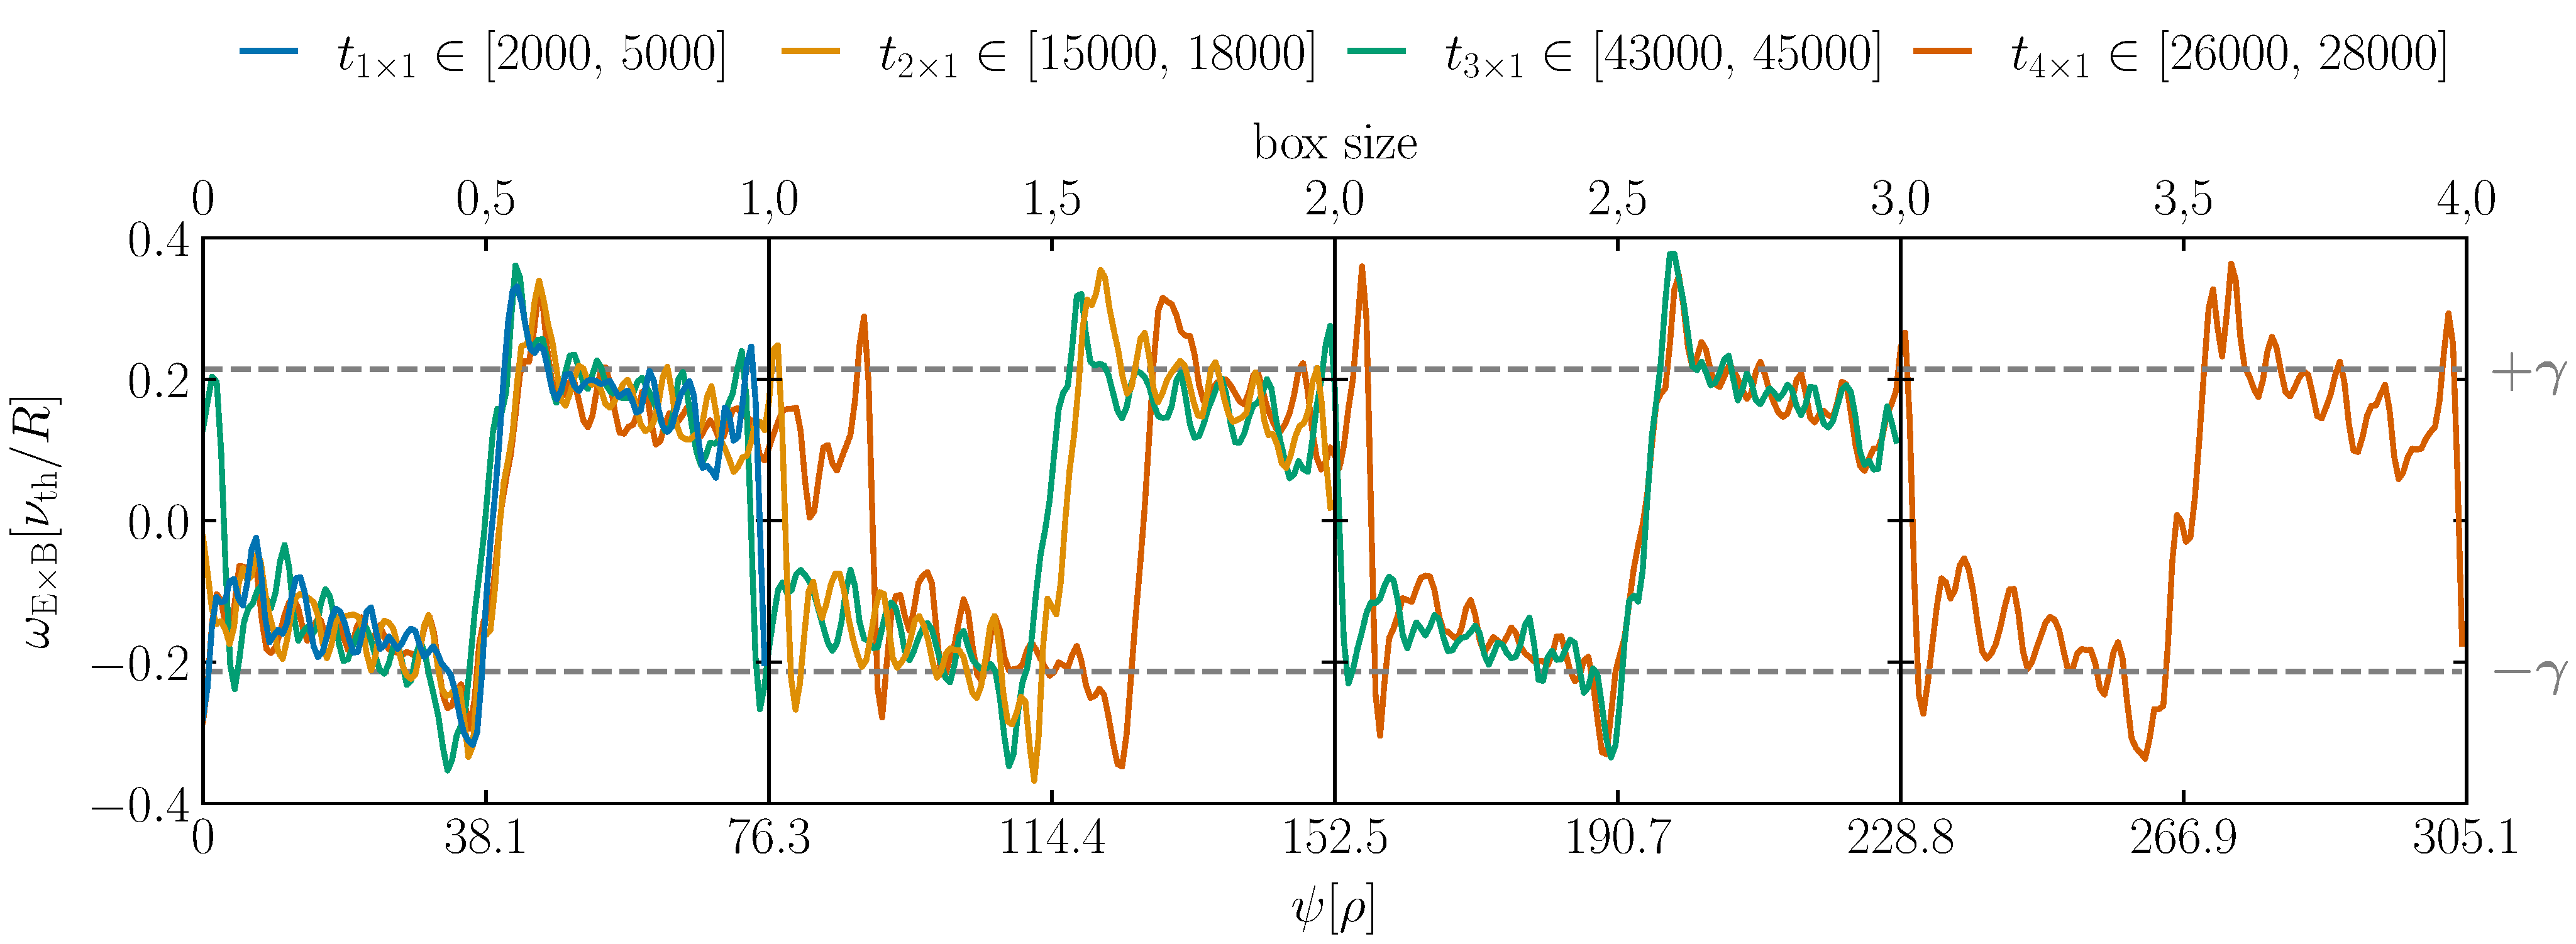
\includegraphics[height = 0.18\paperheight]{Comparison/Boxsize/S6_rlt6.0_boxsize1-2-3-4x1_Ns16_Nvpar48_Nmu9_wexb_comparison.pdf}
	\captionof{figure}{
		Comparison of shearing rate $\wexb$ for the radial box size scan averaged over given a time interval and the growth rate $\pm \gamma$ of the most unstable linear ITG-driven Eigenmode. The staircase structures are radially shifted with respect to each over till alignment for better visibility:\\
		\begin{tabular}{l l l l}
			$t_{1\times 1}$   & $\in [2000, 5000]$,   & $t_{2\times 1}$   & $\in [15000, 18000]$, \\
			$t_{3\times 1}$   & $\in [43000, 45000]$, & $t_{4\times 1}$   & $\in [26000, 28000]$.  \\
		\end{tabular}
	}
	\label{fig:wexb-1-2-3-4x1-compariso}
\end{center}

\newpage
\subsection{Isotropic increased Box Size}
\label{sub:isotropic}

Since the radially elongated simulation domain might inhibit the development of isotropic turbulent structures, in the second test the radial and binormal box size is increased simultaneously.
This scan covers the realizations
\begin{gather*}
	\NR\times\NB \in [1\times1,~1.5\times1.5,~2\times2,~2.5\times2.5,~3\times3]~.
\end{gather*}
Interestingly, suppression of the turbulence by the emergence of a fully developed staircase pattern almost always occurs after $\sim 1000~R/\vth$ [Fig. \ref{fig:eflux-1x1-2x2-3x3-comparison}(a)], i.e., significantly faster compared to the $3\times1$ and $4\times1$ realizations. 
As shown in Fig. \ref{fig:wexb-1x1-2x2-3x3-comparison} or Fig.~\ref{fig:wexb-stable-comparison}(b) this test also confirms the convergence of the staircase pattern size to a typical mesoscale that is distinct from the radial box size in the $\NR > 1$ realizations.

\includegraphicsHere{Comparison/Boxsize/S6_rlt6.0_boxsize1x1-2x2-3x3_Ns16_Nvpar48_Nmu9_comparison_thesis.pdf}{
	\textbf{(a)} Time traces of the heat conduction coefficient $\chi$ for $\rlt = 6.0$ for isotropic increased box sizes,\\
	\textbf{(b)} Time traces of $\hatwexbamp$ for isotropic increased box sizes.
}{fig:eflux-1x1-2x2-3x3-comparison}{}

By contrast to the radial box size scan the $3\times3$ realization shows a stationary pattern with four repetitions of the fully developed staircase structure, i.e., a somewhat smaller pattern size [Fig. \ref{fig:eflux-1x1-2x2-3x3-comparison}(b), Fig. \ref{fig:wexb-1x1-2x2-3x3-comparison} and Fig. \ref{fig:wexb-stable-comparison}(b)]. 
Whether this is related to a possible pattern size dependence on the binormal box size or to the competition between patterns with the two sizes $\lambda \in [57,~ 76]\,\rhoth$ as observed in the first test is addressed in the next paragraph.
The scale of structures developing in the $1.5\times1.5$ and $2.5\times2.5$ realizations (not included in Fig.~\ref{fig:wexb-stable-comparison}, Fig.~\ref{fig:wexb-1x1-2x2-3x3-comparison} and Fig. \ref{fig:eflux-1x1-2x2-3x3-comparison} to preserve the clarity of this figure) also lie within the range given above.

\newpage
\begin{center}
	\captionsetup{type=figure}
	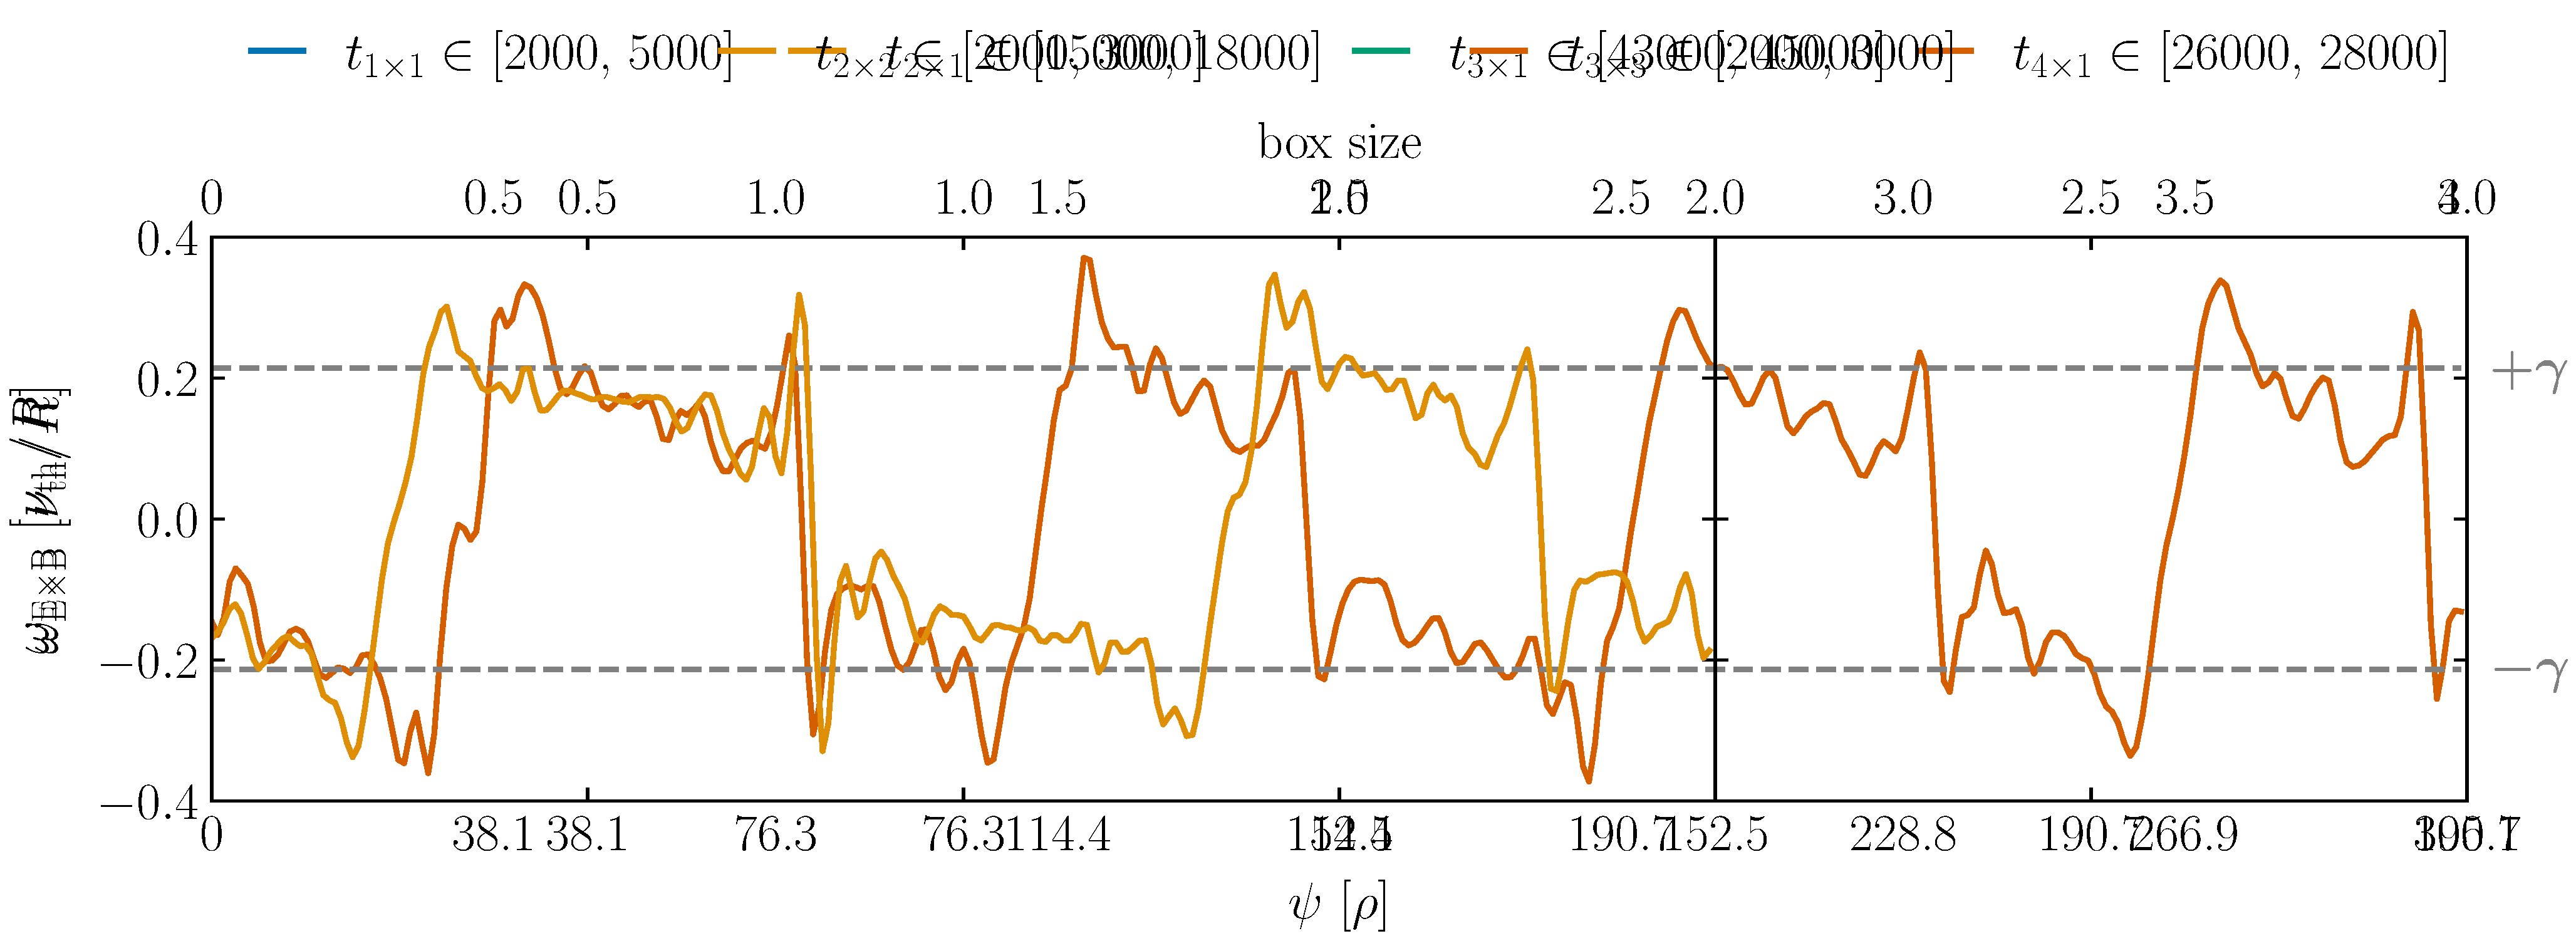
\includegraphics[height = 0.18\paperheight]{Comparison/Boxsize/S6_rlt6.0_boxsize1x1-2x2-3x3_Ns16_Nvpar48_Nmu9_wexb_comparison.pdf}
	\captionof{figure}{
		Comparison of shearing rate $\wexb$ for the isotropic box size scan ($1.5\times1.5$ not $2.5\times2.5$ included) averaged over given a time interval and the growth rate $\pm \gamma$ of the most unstable linear ITG-driven Eigenmode. The staircase structures are radially shifted with respect to each over till alignment for better visibility:\\
		\begin{tabular}{l l l l l l}
			$t_{1\times 1}$   & $\in [2000, 5000]$,   & $t_{2\times 2}$   & $\in [2000, 3000]$,  & $t_{3\times 3}$   & $\in [2000, 3000]$. \\
		\end{tabular}
	}
	\label{fig:wexb-1x1-2x2-3x3-comparison}
\end{center}

Note that two additional realizations of the $3\times3$ case with different initial conditions and otherwise identical parameters confirm structure formation on scales within the range given above [Fig.~\ref{fig:ini-3x3-comparison}].

\begin{center}
	\captionsetup{type=figure}
	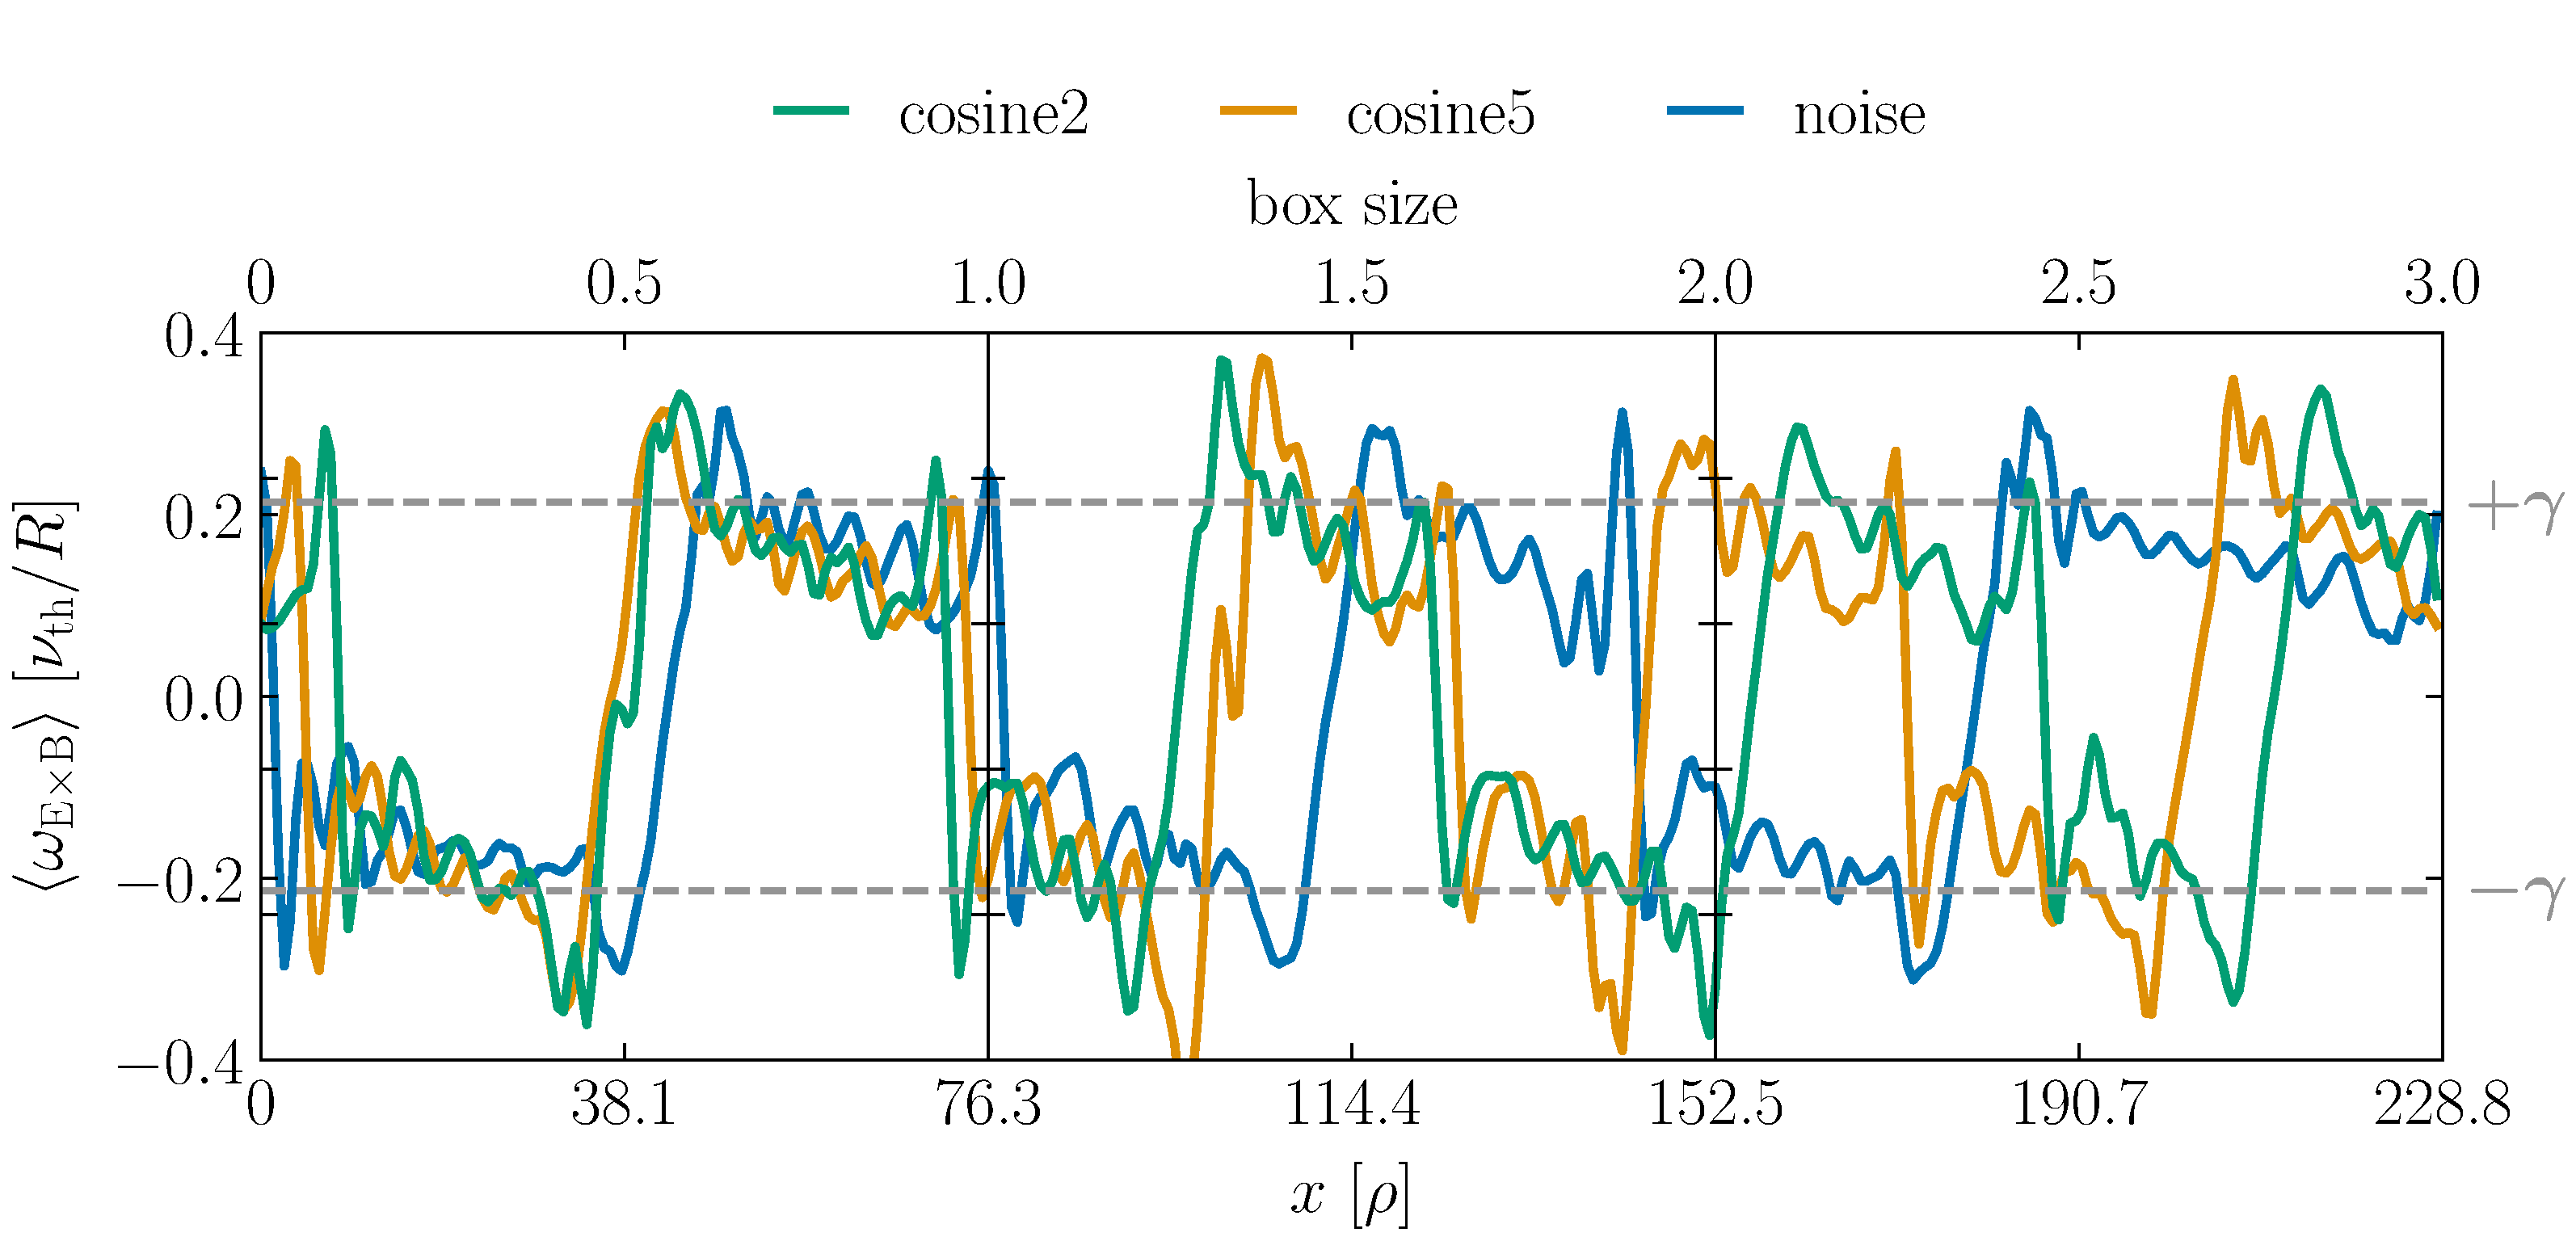
\includegraphics[height = 0.18\paperheight]{Comparison/Boxsize/S6_rlt6.0_boxsize3x3_Ns16_Nvpar48_Nmu9_cosine2-cosine5-noise_wexb_comparison.pdf}
	\captionof{figure}{
		Comparison of shearing rate $\wexb$ for the $3\times3$ box size with different initial conditions averaged over given a time interval and the growth rate $\pm \gamma$ of the most unstable linear ITG-driven Eigenmode. The staircase structures are radially shifted with respect to each over till alignment for better visibility:\\
		\begin{tabular}{l l l l l l}
			$t_\mathrm{cosine2}$   & $\in [2000, 3000]$,   & $t_\mathrm{cosine5}$   & $\in [2000, 3000]$,  & $t_\mathrm{noise}$     & $\in [4000, 5000]$. \\
		\end{tabular}
	}
	\label{fig:ini-3x3-comparison}
\end{center}

\newpage
The negative gradient of the perturbed perpendicular and parallel ion pressure [Fig. \ref{fig:ene-webx-3x3-comparison}] exhibit positive corrugations in regions with maximum $|\wexb|$ and negative corrugations at zero crossings of $\wexb$. 
A radial force balance analysis suggests that the structures in $\wexb$ as depicted in Fig.~\ref{fig:wexb-stable-comparison} are not a consequence of the pressure gradient corrugations as discussed elsewhere \cite{Kosuga2013}.
Rather, the corrugations in the pressure gradient have to be interpreted as a consequence of the staircase structure in $\wexb$ due to the stabilizing zonal flow - turbulence interaction.

\includegraphicsHere{S6_rlt6.0/boxsize3x3/Ns16/Nvpar48/Nmu9/noise/S6_rlt6.0_boxsize3x3_Ns16_Nvpar48_Nmu9_noise_wexb_dens_ene_selection.pdf}{
	Time averaged radial profiles of (top) the $\exb$ shearing rate $\wexb$ and (bottom) the negative gradient of the perpendicular and parallel energy moment $-\langle \nabla_{\!\!x} E_{\perp, \mathrm{i}}\rangle$ and  $-\langle \nabla_{\!\!x} E_{\parallel, \mathrm{i}}\rangle$, respectively, as well as the electric field term $e n_0 \langle \nabla_{\!\!x} \phi\rangle$ of the force balance (on the right axis). Shown is a $3\times3$ realization with $\rlt = 6.0$. Horizontal black and gray bars in the bottom panel indicate the modulation of the negative gradient of the perpendicular energy on the staircase scale.
}{fig:ene-webx-3x3-comparison}{0.8}

\newpage
\subsection{Binormal increased Box Size}
\label{sub:binormal}

In a third test the binormal box size is varied with the radial box size fixed to $\NR = 3$.
This test covers the realizations
\begin{gather*}
	\NR \times \NB \in [3\times1.5,~3\times2.5,~3\times3,~3\times5]~.
\end{gather*}
As in the isotropic scan the turbulence subdued and a fully developed staircase pattern forms after $\sim 2000\,R/\vth$ [Fig.~\ref{fig:eflux-3x1.5-2.5-3-5-comparison}(a)]. The convergence of staircase pattern can be seen in Fig.~\ref{fig:wexb-3x1.5-2.5-3-5-comparison} or Fig.~\ref{fig:wexb-stable-comparison}(c) and confirms again a size of a typical mesoscale. Fig.~\ref{fig:wexb-stable-comparison}(c) also confirms that indeed a competition between patterns with two sizes $\lambda \in [57,~ 76]\,\rhoth$ causing the different results for $3 \times 1$ and $3\times 3$. The zonal flow mode number varies between $\nzf = 3,4$ which can be seen in Fig.~\ref{fig:wexb-stable-comparison}(c) in the $3\times 2.5$ realization. The staircase structure has a pattern between three and four repetitions which get represented in the second repetition with no significant plateau at positive shear. Instead the pattern returns immediately after reaching the maximum shear ($+ \gamma$) to the minimum shear ($- \gamma$) of the third repetition in a steep flank. The Fourier analysis of this case yields no definitely basic mode rather two dominating modes with $\nzf = 3, 4$ with a fraction of the maximum amplitude $\hatwexbamp$ each [Fig. \ref{fig:eflux-3x1.5-2.5-3-5-comparison}(b)].
\includegraphicsHere{Comparison/Boxsize/S6_rlt6.0_boxsize3x1-1.5-2.5-3-5_Ns16_Nvpar48_Nmu9_comparison_thesis.pdf}{
	\textbf{(a)} Time traces of the heat conduction coefficient $\chi$ for $\rlt = 6.0$ for binormal increased box sizes,\\
	\textbf{(b)} Time traces of $\hatwexbamp$ for binormal increased box sizes.
}{fig:eflux-3x1.5-2.5-3-5-comparison}{}\bigskip

\begin{center}
	\captionsetup{type=figure}
	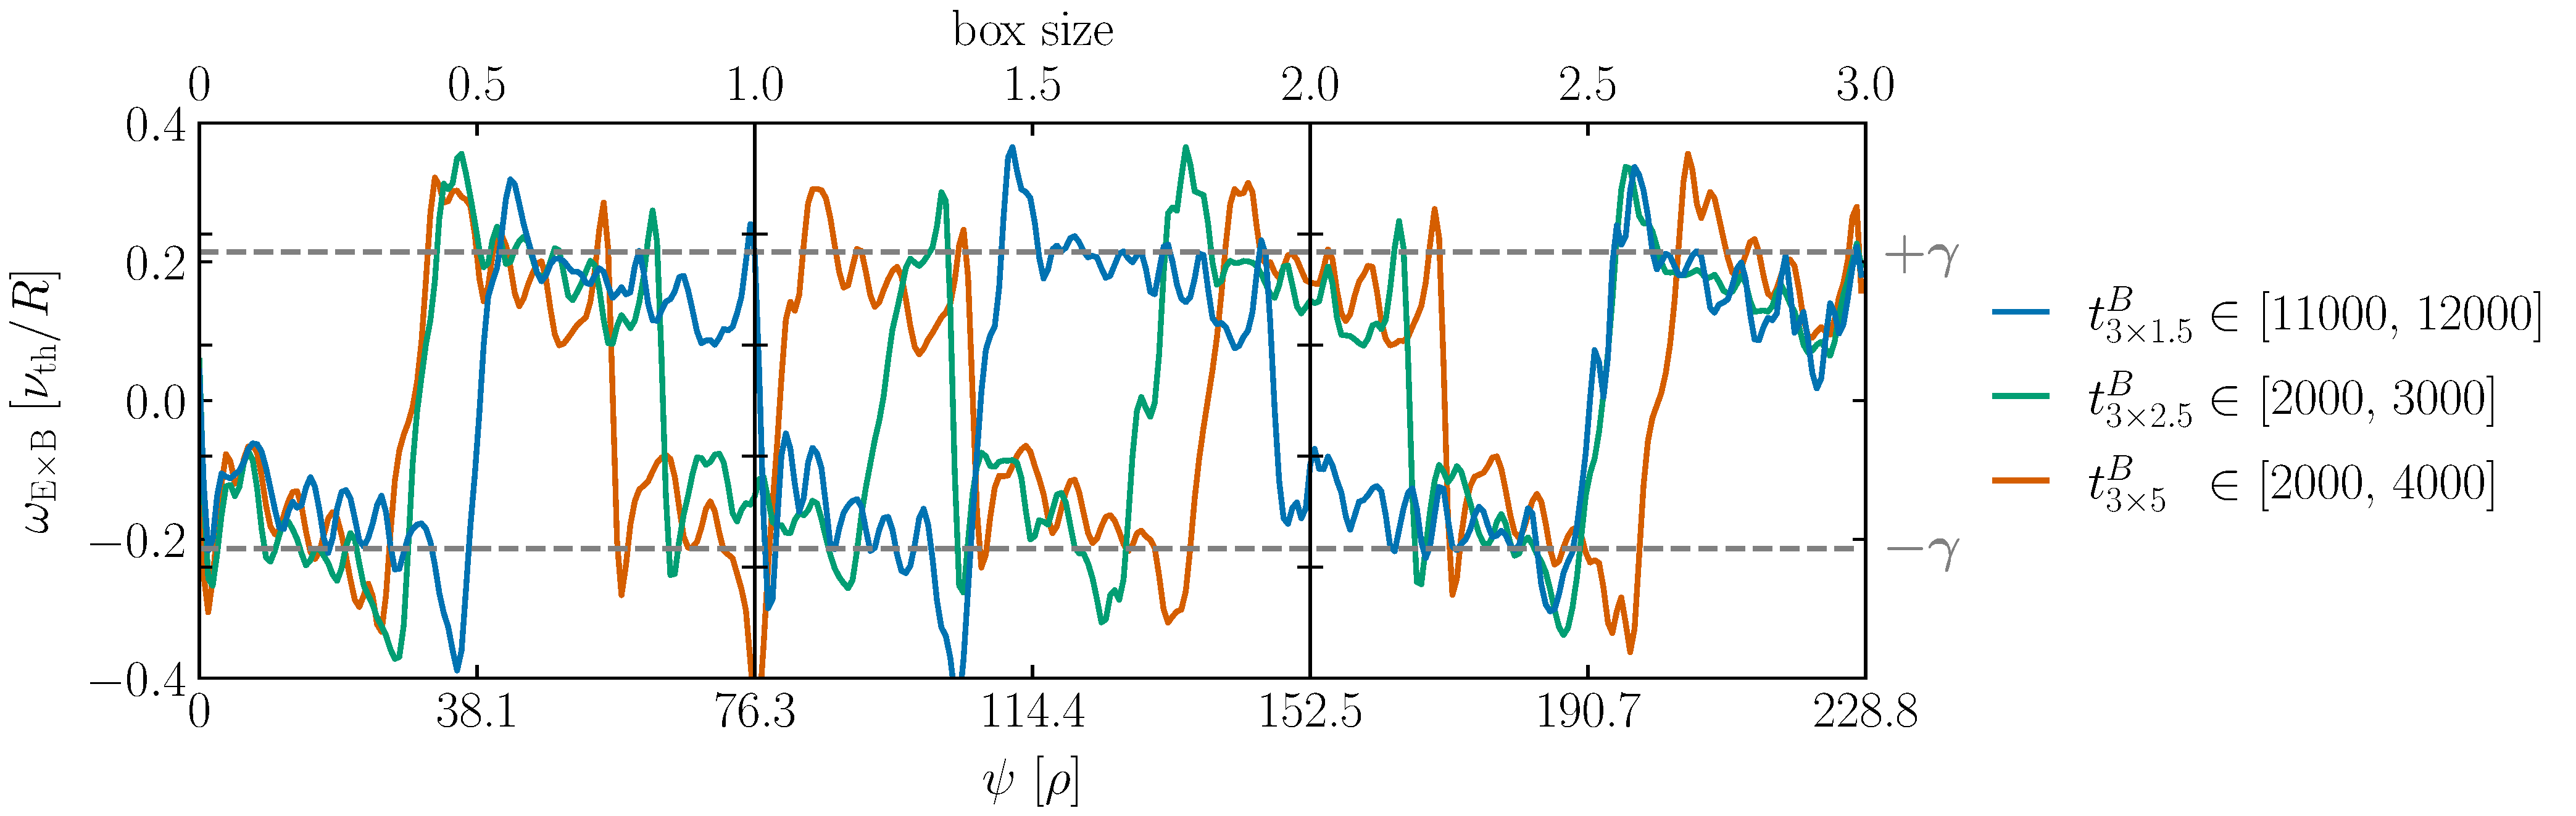
\includegraphics[height = 0.18\paperheight]{Comparison/Boxsize/S6_rlt6.0_boxsize3x1-1.5-2.5-3-5_Ns16_Nvpar48_Nmu9_wexb_comparison.pdf}
	\captionof{figure}{
		Comparison of shearing rate $\wexb$ for the binormal box size scan averaged over given a time interval and the growth rate $\pm \gamma$ of the most unstable linear ITG-driven Eigenmode. The staircase structures are radially shifted with respect to each over till alignment for better visibility:\\
		\begin{tabular}{l l l l}
			$t_{3\times 1.5}$ & $\in [2000, 3000]$,   & $t_{3\times 2.5}$ & $\in [2000, 3000]$,   \\
		    $t_{3\times 3}$   & $\in [2000, 3000]$,   & $t_{3\times 5}$   & $\in [1000, 3000]$.    \\
		\end{tabular}
	}
	\label{fig:wexb-3x1.5-2.5-3-5-comparison}
\end{center}

\newpage

\subsection{Staircase Structures in Comparison}
\label{sub:comparisonwexb}

\includegraphicsHere{Comparison/Boxsize/S6_rlt6.0_boxsize1-2-3-4x1-1.5-2-2.5-3-5_Ns16_Nvpar48_Nmu9_wexb_comparison_thesis.pdf}{
	Comparison of shearing rate $\wexb$ for each box size scan averaged over given a time interval and the growth rate $\pm \gamma$ of the most unstable linear ITG-driven Eigenmode. The staircase structures are radially shifted with respect to each over till alignment for better visibility:\\
	\begin{tabular}{l l l l l}
		\textbf{(a) radial:}    & $t_{1\times 1}$   & $\in [2000, 5000]$,   & $t_{2\times 1}$   & $\in [15000, 18000]$, \\
		                        & $t_{3\times 1}$   & $\in [43000, 45000]$, & $t_{4\times 1}$   & $\in [26000, 28000]$; \\
		\textbf{(b) isotropic:} & $t_{1\times 1}$   & $\in [2000, 5000]$,   & $t_{2\times 2}$   & $\in [2000, 3000]$,   \\
		                        & $t_{3\times 3}$   & $\in [2000, 3000]$;   &                   &                       \\
		\textbf{(c) binormal:}  & $t_{3\times 1.5}$ & $\in [2000, 3000]$,   & $t_{3\times 2.5}$ & $\in [2000, 3000]$,   \\
		                        & $t_{3\times 3}$   & $\in [2000, 3000]$,   & $t_{3\times 5}$   & $\in [1000, 3000]$.   \\
	\end{tabular}
}{fig:wexb-stable-comparison}{}